\documentclass{ximera}

\usepackage{epsfig}

\graphicspath{
  {./}
  {figures/}
}

\usepackage{epstopdf}
%\usepackage{ulem}
\usepackage[normalem]{ulem}

\epstopdfsetup{outdir=./}

\usepackage{morewrites}
\makeatletter
\newcommand\subfile[1]{%
\renewcommand{\input}[1]{}%
\begingroup\skip@preamble\otherinput{#1}\endgroup\par\vspace{\topsep}
\let\input\otherinput}
\makeatother

\newcommand{\EXER}{}
\newcommand{\includeexercises}{\EXER\directlua{dofile(kpse.find_file("exercises","lua"))}}

\newenvironment{computerExercise}{\begin{exercise}}{\end{exercise}}

%\newcounter{ccounter}
%\setcounter{ccounter}{1}
%\newcommand{\Chapter}[1]{\setcounter{chapter}{\arabic{ccounter}}\chapter{#1}\addtocounter{ccounter}{1}}

%\newcommand{\section}[1]{\section{#1}\setcounter{thm}{0}\setcounter{equation}{0}}

%\renewcommand{\theequation}{\arabic{chapter}.\arabic{section}.\arabic{equation}}
%\renewcommand{\thefigure}{\arabic{chapter}.\arabic{figure}}
%\renewcommand{\thetable}{\arabic{chapter}.\arabic{table}}

%\newcommand{\Sec}[2]{\section{#1}\markright{\arabic{ccounter}.\arabic{section}.#2}\setcounter{equation}{0}\setcounter{thm}{0}\setcounter{figure}{0}}
  
\newcommand{\Sec}[2]{\section{#1}}

\setcounter{secnumdepth}{2}
%\setcounter{secnumdepth}{1} 

%\newcounter{THM}
%\renewcommand{\theTHM}{\arabic{chapter}.\arabic{section}}

\newcommand{\trademark}{{R\!\!\!\!\!\bigcirc}}
%\newtheorem{exercise}{}

\newcommand{\dfield}{{\sf SlopeField}}

\newcommand{\pplane}{{\sf PhasePlane}}

\newcommand{\PPLANE}{{\sf PHASEPLANE}}

% BADBAD: \newcommand{\Bbb}{\bf}. % Package amsfonts Warning: Obsolete command \Bbb; \mathbb should be used instead.

\newcommand{\R}{\mbox{$\mathbb{R}$}}
\let\C\relax
\newcommand{\C}{\mbox{$\mathbb{C}$}}
\newcommand{\Z}{\mbox{$\mathbb{Z}$}}
\newcommand{\N}{\mbox{$\mathbb{N}$}}
\newcommand{\D}{\mbox{{\bf D}}}

\newcommand{\WW}{\mathcal{W}}

\usepackage{amssymb}
%\newcommand{\qed}{\hfill\mbox{\raggedright$\square$} \vspace{1ex}}
%\newcommand{\proof}{\noindent {\bf Proof:} \hspace{0.1in}}

\newcommand{\setmin}{\;\mbox{--}\;}
\newcommand{\Matlab}{{M\small{AT\-LAB}} }
\newcommand{\Matlabp}{{M\small{AT\-LAB}}}
\newcommand{\computer}{\Matlab Instructions}
\renewcommand{\computer}{M\small{ATLAB} Instructions}
\newcommand{\half}{\mbox{$\frac{1}{2}$}}
\newcommand{\compose}{\raisebox{.15ex}{\mbox{{\scriptsize$\circ$}}}}
\newcommand{\AND}{\quad\mbox{and}\quad}
\newcommand{\vect}[2]{\left(\begin{array}{c} #1_1 \\ \vdots \\
 #1_{#2}\end{array}\right)}
\newcommand{\mattwo}[4]{\left(\begin{array}{rr} #1 & #2\\ #3
&#4\end{array}\right)}
\newcommand{\mattwoc}[4]{\left(\begin{array}{cc} #1 & #2\\ #3
&#4\end{array}\right)}
\newcommand{\vectwo}[2]{\left(\begin{array}{r} #1 \\ #2\end{array}\right)}
\newcommand{\vectwoc}[2]{\left(\begin{array}{c} #1 \\ #2\end{array}\right)}

\newcommand{\ignore}[1]{}


\newcommand{\inv}{^{-1}}
\newcommand{\CC}{{\cal C}}
\newcommand{\CCone}{\CC^1}
\newcommand{\Span}{{\rm span}}
\newcommand{\rank}{{\rm rank}}
\newcommand{\trace}{{\rm tr}}
\newcommand{\RE}{{\rm Re}}
\newcommand{\IM}{{\rm Im}}
\newcommand{\nulls}{{\rm null\;space}}

\newcommand{\dps}{\displaystyle}
\newcommand{\arraystart}{\renewcommand{\arraystretch}{1.8}}
\newcommand{\arrayfinish}{\renewcommand{\arraystretch}{1.2}}
\newcommand{\Start}[1]{\vspace{0.08in}\noindent {\bf Section~\ref{#1}}}
\newcommand{\exer}[1]{\noindent {\bf \ref{#1}}}
\newcommand{\ans}{\textbf{Answer:} }
\newcommand{\matthree}[9]{\left(\begin{array}{rrr} #1 & #2 & #3 \\ #4 & #5 & #6
\\ #7 & #8 & #9\end{array}\right)}
\newcommand{\cvectwo}[2]{\left(\begin{array}{c} #1 \\ #2\end{array}\right)}
\newcommand{\cmatthree}[9]{\left(\begin{array}{ccc} #1 & #2 & #3 \\ #4 & #5 &
#6 \\ #7 & #8 & #9\end{array}\right)}
\newcommand{\vecthree}[3]{\left(\begin{array}{r} #1 \\ #2 \\
#3\end{array}\right)}
\newcommand{\cvecthree}[3]{\left(\begin{array}{c} #1 \\ #2 \\
#3\end{array}\right)}
\newcommand{\cmattwo}[4]{\left(\begin{array}{cc} #1 & #2\\ #3
&#4\end{array}\right)}

\newcommand{\Matrix}[1]{\ensuremath{\left(\begin{array}{rrrrrrrrrrrrrrrrrr} #1 \end{array}\right)}}

\newcommand{\Matrixc}[1]{\ensuremath{\left(\begin{array}{cccccccccccc} #1 \end{array}\right)}}



\renewcommand{\labelenumi}{\theenumi}
\newenvironment{enumeratea}%
{\begingroup
 \renewcommand{\theenumi}{\alph{enumi}}
 \renewcommand{\labelenumi}{(\theenumi)}
 \begin{enumerate}}
 {\end{enumerate}
 \endgroup}

\newcounter{help}
\renewcommand{\thehelp}{\thesection.\arabic{equation}}

%\newenvironment{equation*}%
%{\renewcommand\endequation{\eqno (\theequation)* $$}%
%   \begin{equation}}%
%   {\end{equation}\renewcommand\endequation{\eqno \@eqnnum
%$$\global\@ignoretrue}}

%\input{psfig.tex}

\author{Martin Golubitsky and Michael Dellnitz}

%\newenvironment{matlabEquation}%
%{\renewcommand\endequation{\eqno (\theequation*) $$}%
%   \begin{equation}}%
%   {\end{equation}\renewcommand\endequation{\eqno \@eqnnum
% $$\global\@ignoretrue}}

\newcommand{\soln}{\textbf{Solution:} }
\newcommand{\exercap}[1]{\centerline{Figure~\ref{#1}}}
\newcommand{\exercaptwo}[1]{\centerline{Figure~\ref{#1}a\hspace{2.1in}
Figure~\ref{#1}b}}
\newcommand{\exercapthree}[1]{\centerline{Figure~\ref{#1}a\hspace{1.2in}
Figure~\ref{#1}b\hspace{1.2in}Figure~\ref{#1}c}}
\newcommand{\para}{\hspace{0.4in}}

\usepackage{ifluatex}
\ifluatex
\ifcsname displaysolutions\endcsname%
\else
\renewenvironment{solution}{\suppress}{\endsuppress}
\fi
\else
\renewenvironment{solution}{}{}
\fi

\ifcsname answer\endcsname
\renewcommand{\answer}{}
\fi

%\ifxake
%\newenvironment{matlabEquation}{\begin{equation}}{\end{equation}}
%\else
\newenvironment{matlabEquation}%
{\let\oldtheequation\theequation\renewcommand{\theequation}{\oldtheequation*}\begin{equation}}%
  {\end{equation}\let\theequation\oldtheequation}
%\fi

\makeatother

\newcommand{\RED}[1]{{\color{red}{#1}}} 


\title{Hopf Bifurcations Revisited}

\begin{document}
\begin{abstract}
\end{abstract}
\maketitle


\label{S:HopfBif}
\index{bifurcation!Hopf}

As discussed in Section~\ref{S:bifurcation}, Hopf bifurcation occurs at
an equilibrium when the Jacobian $J$ has a pair of complex conjugate, purely 
imaginary eigenvalues, that is, when $\trace(J)=0$ and $\det(J)>0$.  In two 
dimensions, $J$ is a center and the phase portrait of the linearized equation 
consists of a continuous family of periodic solutions.  The Hopf bifurcation 
theorem states that under reasonable assumptions this family of periodic 
solutions persists in the nonlinear equations.   \index{periodic solution}

Since $J$ is invertible, the (two dimensional) implicit function theorem 
guarantees that there is a curve of equilibria with one equilibrium for 
each value $\rho$ near the bifurcation value.  Because of this, it makes 
sense to ask how the real parts of the eigenvalues of the Jacobian are 
changing as $\rho$ varies.  The basic assumption that we make about Hopf 
bifurcation is that the real parts of the eigenvalues of the Jacobian go 
through zero with nonzero speed.  We can rewrite this condition algebraically 
as follows.  Let $X(\rho)$ denote the curve of equilibria and $J_{X(\rho)}$ 
the corresponding Jacobian matrix.  Then, the real part of the complex 
conjugate eigenvalues of the Jacobian matrix is: 
\index{eigenvalue crossing condition}
\[
\frac{1}{2}\trace(J_{X(\rho)}). 
\]
The condition that the real parts of the eigenvalues cross through 
zero with nonzero speed is:
\begin{equation}  \label{e:2dhopf}
\frac{d}{d\rho} \trace(J_{X(\rho)}) \neq 0.
\end{equation}
Condition \eqref{e:2dhopf} is called the {\em eigenvalue crossing condition\/}.


\subsection*{Two Examples}

As a first example, consider the linear system
\begin{matlabEquation}  \label{e:Hopflin}
\begin{array}{rcl}
\dot{x} & = & \rho x - y \\
\dot{y} & = & x + \rho y.
\end{array}
\end{matlabEquation}
It is easy to check that $\trace(J)=2\rho$ and that \eqref{e:2dhopf}
is satisfied.  Note that the origin is a spiral sink when $\rho<0$ 
and a spiral source when $\rho>0$.  When $\rho=0$, the origin is a
center, and there is a continuous family of periodic solutions
surrounding this center.  See Figure~\ref{F:Hopfabc}

\begin{figure*}[htb]
           \centerline{%
           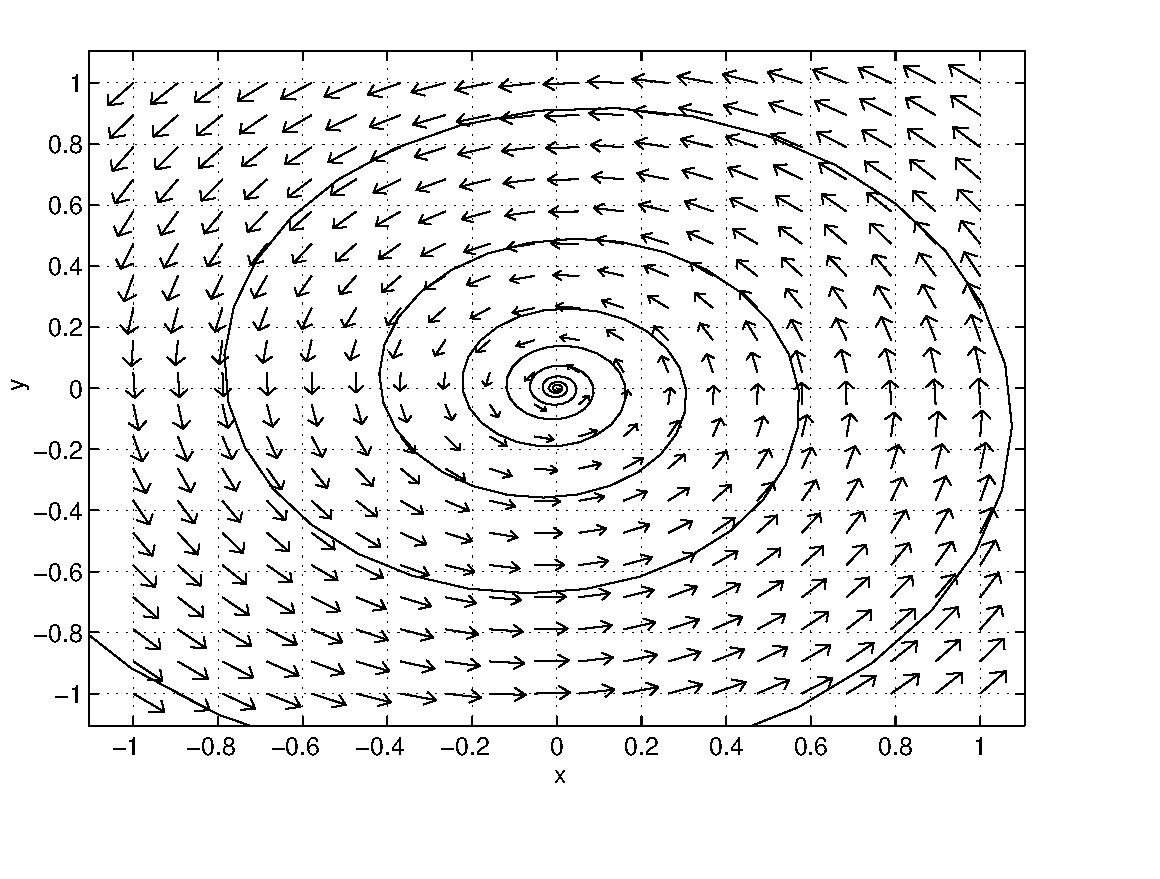
\includegraphics[width=2.3in]{../figures/hopfa.pdf}
           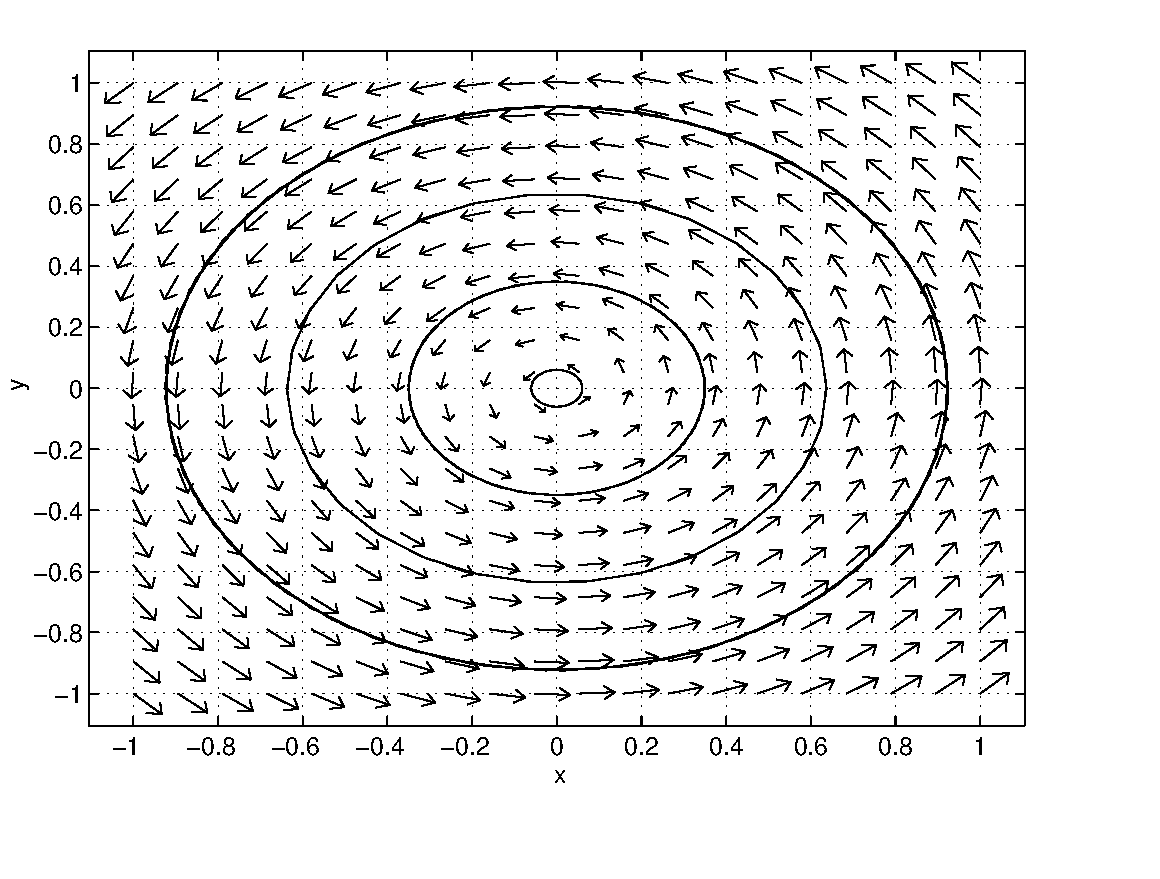
\includegraphics[width=2.3in]{../figures/hopfb.pdf} 
           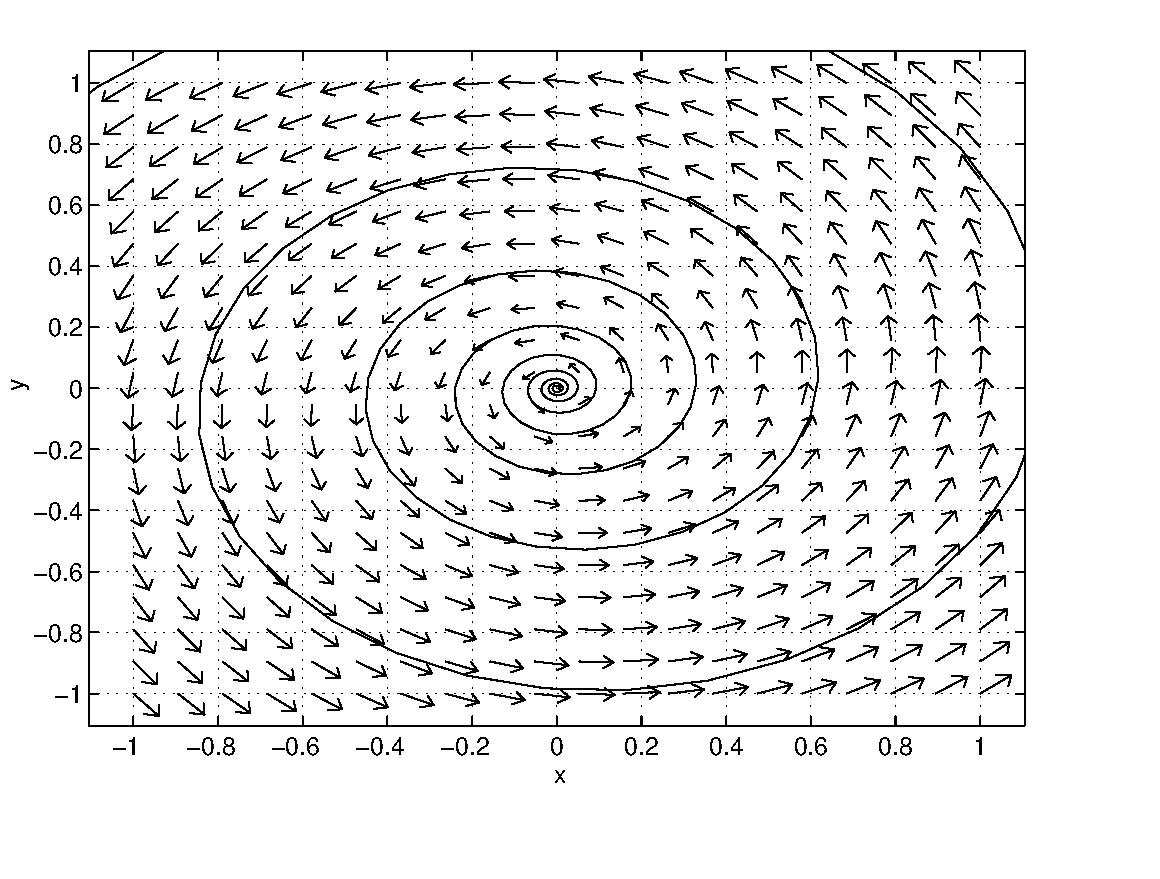
\includegraphics[width=2.3in]{../figures/hopfc.pdf}}
	\vspace*{-0.2in}
	\hspace{0.3in} $\rho=-0.1$  \hspace{1.7in} $\rho=0$
		\hspace{1.8in} $\rho=0.1$ 
           \caption{Phase planes for \protect\eqref{e:Hopflin}.}
           \label{F:Hopfabc}
\end{figure*}


As a second example, consider the predator-prey Volterra-Lotka 
equations \eqref{e:pop3}.  These equations are: \index{Volterra-Lotka equations}
\begin{equation} \label{e:pop3a}
\begin{array}{rcl}
\dot{x} & = & x(\mu + \rho x -       y) \\
\dot{y} & = & y( -1 +       x).
\end{array}
\end{equation}   
We fix $\mu>0$ and vary the parameter $\rho$.  Our previous 
calculations showed that \eqref{e:pop3a} has a center when 
$\rho=0$.  Indeed, these equations have a nontrivial equilibrium 
at $(x_0,y_0)=(1, \mu+\rho)$.  So $X(\rho)=(1,\mu+\rho)$.

The Jacobian matrix of \eqref{e:pop3a} is
\[
J_{(x,y)} = \left(\begin{array}{cc} \mu + 2\rho x - y & -x \\
y & -1 + x \end{array}\right).
\]
Evaluating $J$ along the equilibria $X(\rho)$ yields
\[
J_{(1,\mu+\rho)} = \left(\begin{array}{cc} \rho & -1 \\
\mu+\rho & 0 \end{array}\right).
\]
It follows that
\[
\trace(J_{X(\rho)}) = \rho,
\]
and hence 
\[
\frac{d}{d\rho} \trace(J_{X(\rho)}) = 1 \neq 0.
\]
So the eigenvalue crossing condition is satisfied for equation 
\eqref{e:pop3a}.  

\begin{theorem}[simple Hopf bifurcation]  \label{T:2dhopf}
Suppose that the system of differential equations \eqref{e:2deqn}
has a point of Hopf bifurcation at $(X_0,\rho_0)$.  Suppose, in 
addition, that the 
eigenvalue crossing\index{eigenvalue crossing condition} 
condition \eqref{e:2dhopf} 
is satisfied.  Then there exists a unique branch of periodic 
solutions to \eqref{e:2deqn} emanating from $(X_0,\rho_0)$. 

Moreover, every periodic solution to \eqref{e:2deqn} that occurs for
a parameter value $\rho$ near $\rho_0$ and in phase space near $X_0$ 
is included in this branch of periodic solutions.
\end{theorem}  \index{bifurcation!Hopf}

Recall that the predator-prey equations are obtained from \eqref{e:pop3a}
by setting $\rho=0$.  We have seen in our numerical analysis of the 
predator-prey equations that for all values of $\mu>0$ there is a center 
surrounded by a continuous family of periodic solutions.  (We 
have not proved this fact, but it is true.)  Since the eigenvalue 
crossing condition is satisfied for the predator-prey Volterra-Lotka 
equations, it follows from the simple Hopf bifurcation theorem that 
there are no other periodic solutions near the bifurcation point. 
\index{predator-prey equation}  Indeed, the numerical computations 
shown in Figure~\ref{F:pop3} support this conclusion.

\subsection*{A Significant Effect of Nonlinearity}

The most important point about the periodic solutions guaranteed by 
Theorem~\ref{T:2dhopf} is that they need not occur at the same parameter 
value. For example, in the CSTR there is an isolated limit cycle for each 
value of $\rho$ on one side of the bifurcation value.  See the numerical 
calculations of the CSTR in Figure~\ref{F:CSTR} for $\rho=0.545$ where an
isolated limit cycle is observed, and $\rho=0.520$ where no periodic
solution is seen. \index{CSTR}

Indeed, the CSTR equations behave more typically than the 
Volterra-Lotka equations.  What we expect to happen at a Hopf bifurcation 
point is summarized by the bifurcation diagrams of Figures~\ref{F:hopf} and 
\ref{F:hopf2}.  In these figures we see a single branch of periodic solutions 
emanating from the Hopf bifurcation point either 
{\em supercritically\/}\index{bifurcation!supercritical} (for 
values of $\rho$ greater than the one where Hopf bifurcation occurs) or 
{\em subcritically\/}\index{bifurcation!subcritical} 
(for values of $\rho$ less than the critical Hopf bifurcation value).

\begin{figure}[htb]
           \centerline{%
	   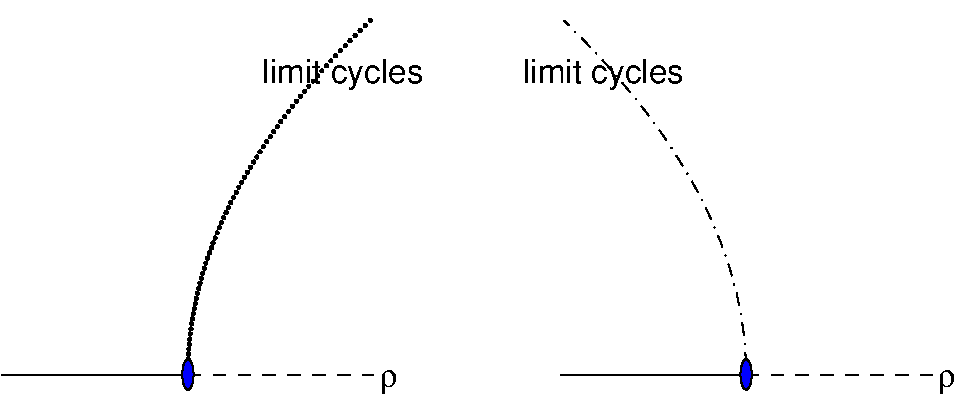
\includegraphics[height=1.7in]{../figures/Hopfbif1a.pdf}}
           \caption{Typical bifurcation diagrams for Hopf bifurcation.}
           \label{F:hopf}
\end{figure}

\begin{figure}[htb]
           \centerline{%
	   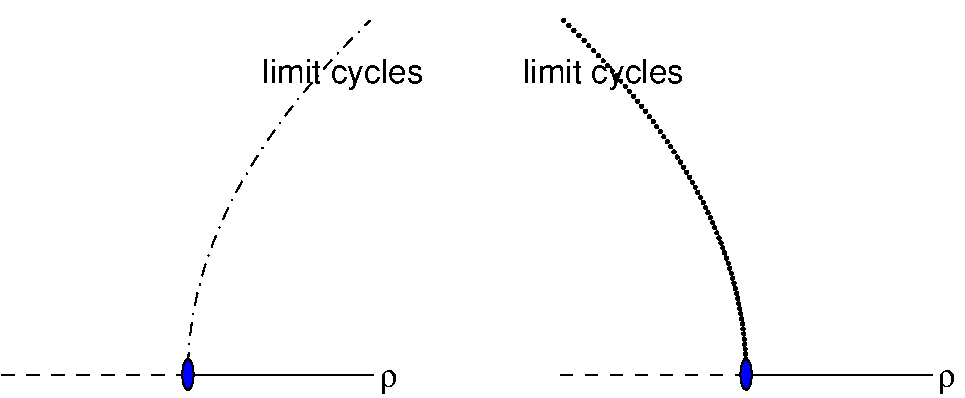
\includegraphics[height=1.7in]{../figures/Hopfbif1b.pdf}}
           \caption{Typical bifurcation diagrams for Hopf bifurcation.}
           \label{F:hopf2}
\end{figure}

\subsubsection*{Exchange of Stability}
\index{stability!exchange of}

Assume that the equilibrium solution is stable at values below the 
bifurcation value and that the eigenvalue crossing condition \eqref{e:2dhopf} 
holds.  Then typically the periodic solutions will appear above 
the bifurcation value and be asymptotically 
stable\index{stability!asymptotic} or they will 
appear below the bifurcation value and be unstable.  Which one of these 
scenarios actually occurs depends on the sign of a certain coefficient 
computed from the second and third order terms of the differential equation.  
This coefficient plays the same role in Hopf bifurcation that condition 
\eqref{e:2dbifur} plays in saddle-node bifurcations.  The coefficient is 
much more complicated than \eqref{e:2dbifur} and we do not attempt to give 
its explicit form here.

If, on the other hand, the equilibrium solution is unstable at values below 
the bifurcation value, then the periodic solutions will be unstable when
supercritical and stable when subcritical.  See Figure~\ref{F:hopf2}.  In 
particular, the periodic solutions are stable only when they appear on the 
opposite side of criticality from the stable equilibrium.  This phenomenon 
is called {\em exchange of stability\/}.

\subsubsection*{Hopf Bifurcation in Phase-Amplitude Equations}

We can understand how typical Hopf bifurcations behave by looking at
phase-ampli\-tude equations of ODEs. The system is:  
\index{phase-amplitude equations}
\begin{matlabEquation}  \label{e:nonlinhopf}
\frac{d}{dt}\vectwo{x}{y} = (\rho +a(x^2+y^2))\vectwo{x}{y} + \vectwo{-y}{x}.
\end{matlabEquation}
In amplitude $r$ and phase $\theta$, \eqref{e:nonlinhopf} becomes
\begin{eqnarray*}
\dot{r} & = & (\rho+ar^2)r \\
\dot{\theta} & = & 1.
\end{eqnarray*}
The nontrivial zeros of the amplitude equation --- which correspond to 
periodic solutions in the original system --- are 
\[
\rho = -a r^2.
\]
It follows that there is one periodic trajectory of \eqref{e:nonlinhopf}
for $\rho>0$ when $a<0$ and for $\rho<0$ when $a>0$.  
Phase portraits for \eqref{e:nonlinhopf} when $a=-1$ are presented in 
Figure~\ref{F:nonlinhopf}.  Note the existence of a stable limit 
cycle\index{limit cycle!stable}
when $\rho>0$ and the slowness of the convergence of trajectories 
to the origin when $\rho=0$.

\begin{figure*}[htb]
           \centerline{%
           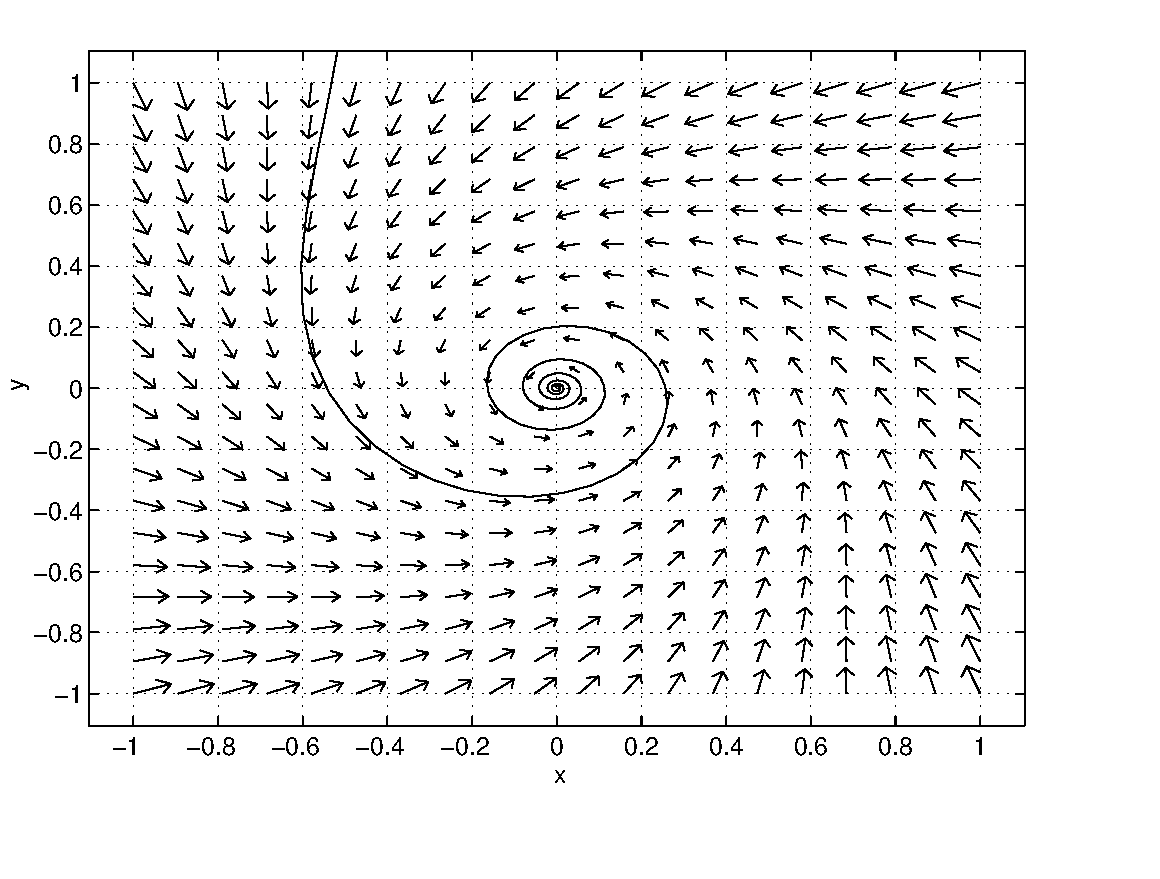
\includegraphics[width=2.3in]{../figures/hopfna.pdf}
           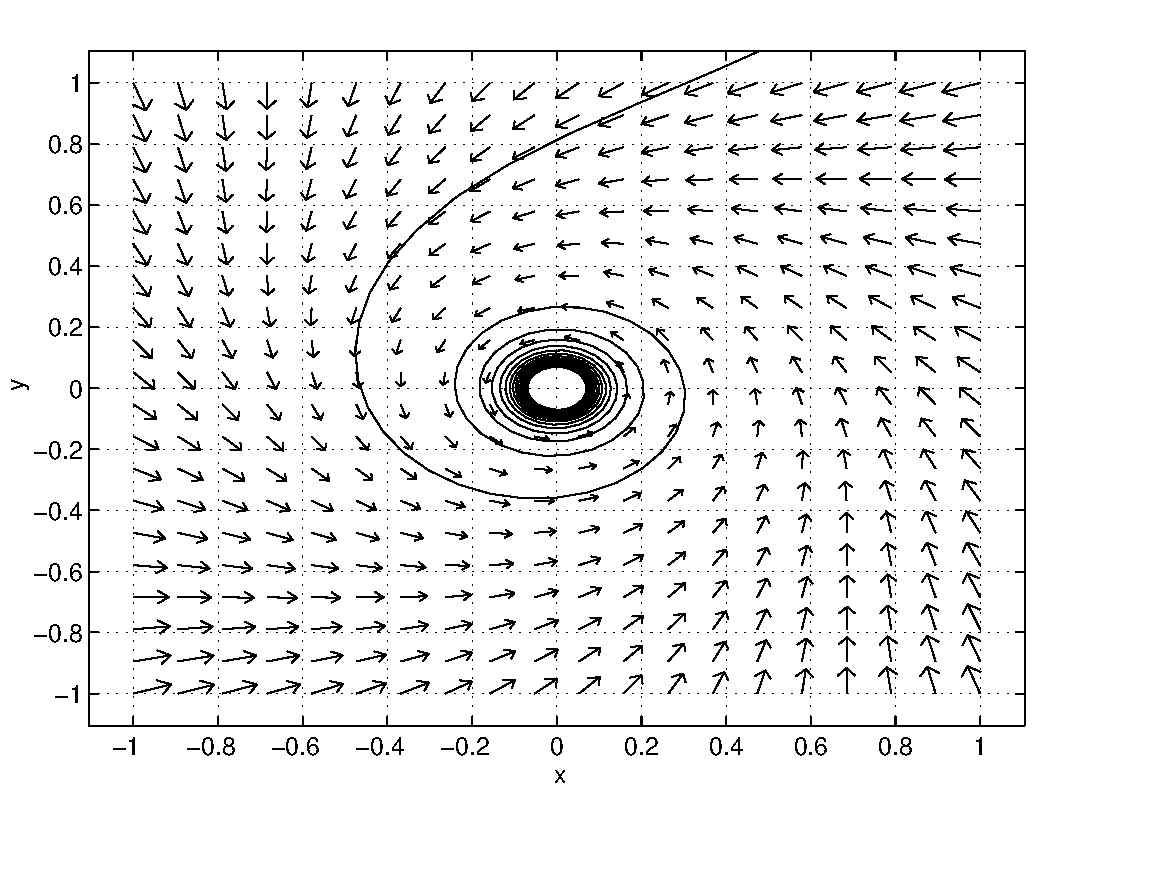
\includegraphics[width=2.3in]{../figures/hopfnb.pdf} 
           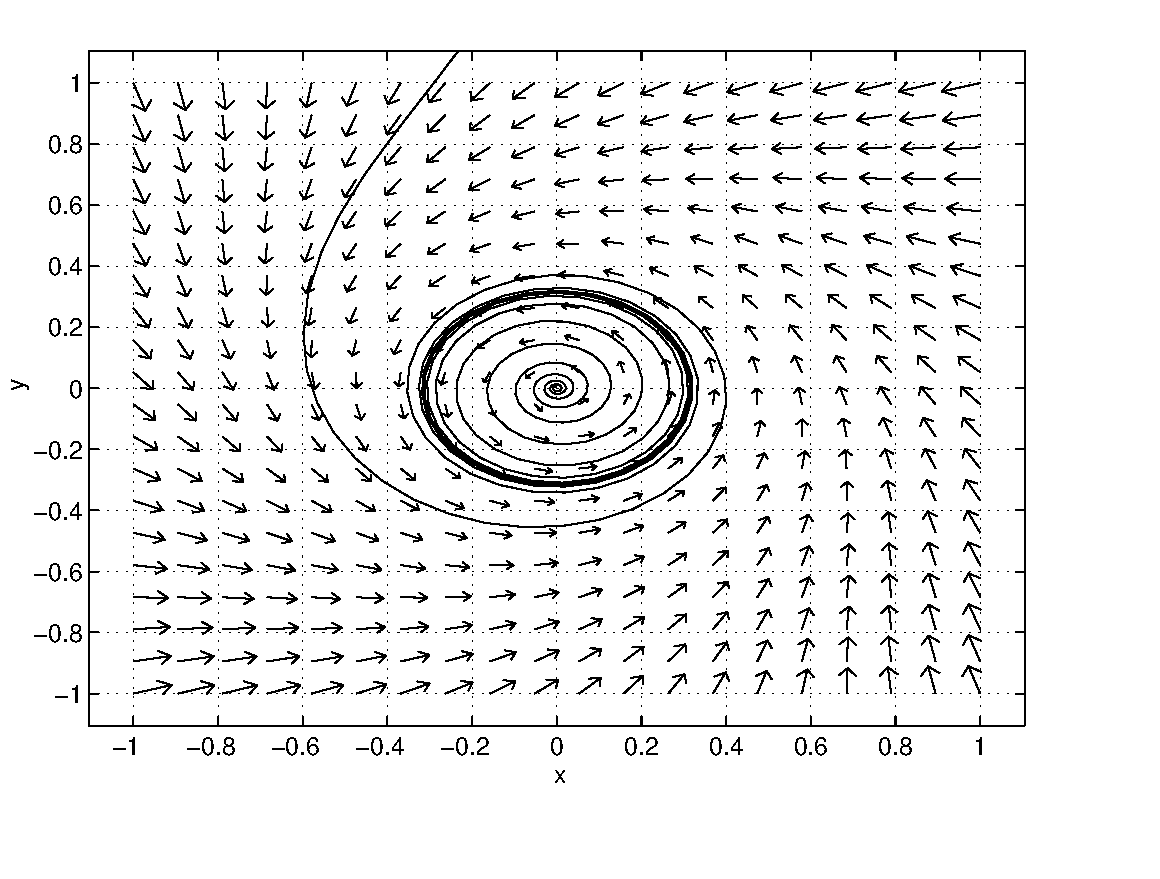
\includegraphics[width=2.3in]{../figures/hopfnc.pdf}}
 	\vspace*{-0.2in}
	\hspace{0.3in} $\rho=-0.1$  \hspace{1.7in} $\rho=0$
		\hspace{1.8in} $\rho=0.1$ 
          \caption{Phase planes for \protect\eqref{e:nonlinhopf} with $a=-1$.}
           \label{F:nonlinhopf}
\end{figure*}





\includeexercises


































\end{document}
